%%%%%%%%%%%%%%%%%%%%%%%%%%%%%%%

\section{Invariant $B$ mass fit and Dalitz plot distributions} 
\label{sec:MassFit}
%\color{red}{code is hepfarm20:/projects/lhcb/users/zhangyx/PcFit/Lb2JpsiPH/Macro/MassFit/MassFit.C, root -l run.C}

\subsection{Signal yields}
After the selections, 
the sample of ${B}^{+} \rightarrow {J} / {\psi} {\phi} {K}^{+}$ candidates consists of the signal and of the combinatorial background.
Figure.~\ref{fig:MassFit_run} show the fitted invariant mass distribution of the ${B}^{+} \rightarrow {J} / {\psi} {\phi} {K}^{+}$  candidates, 
for Run 1 and Run 2 separately. 
The signal shape is described by an Hypatia function. %an alternative fit with the Hypatia model is also performed; 
The shape of the combinatorial background is described by the second order Chebyshev polynomial function. 
In $\pm15$\mev signal region around the $\Bp$ peak,
the signal yield is $5043\pm77$ ($19176\pm147$), 
and the combinatorial background yield is $275\pm10$ ($738\pm17$) for Run 1 (Run 2).
Background fraction is 5.2\% (3.7\%) for Run 1 (Run 2), overall 4.0\%. 
Due to loosen the $\chisqip$ selection of the kaon candidates from $>9$ to $>4$, 20\% signal gain is achieved compared to the Run 1 publication. 
Also due to more input variables used in MVA (\eg $\ProbNN{\rm k}$ and $\chi^2_{\rm FD}$), 
the background fraction is significantly reduced from 27\% to 5\% (Run 1). 
The multiple candidate fraction is 0.9\% in a $B$ mass range of 5220-5360\mev. 
%%%%%%%%%%%%%%%%%%%%%%%%%%%%%%%%%%%%%%%%%%%%%%%%%%%%%%%%%%%%%%%%%%%%%%%%%%%%%%%%%%%%%%%%%%%%%%%%%%%%%%%%%%%%%%%%%%%%%%%
\begin{figure}[!tbp]
\centering
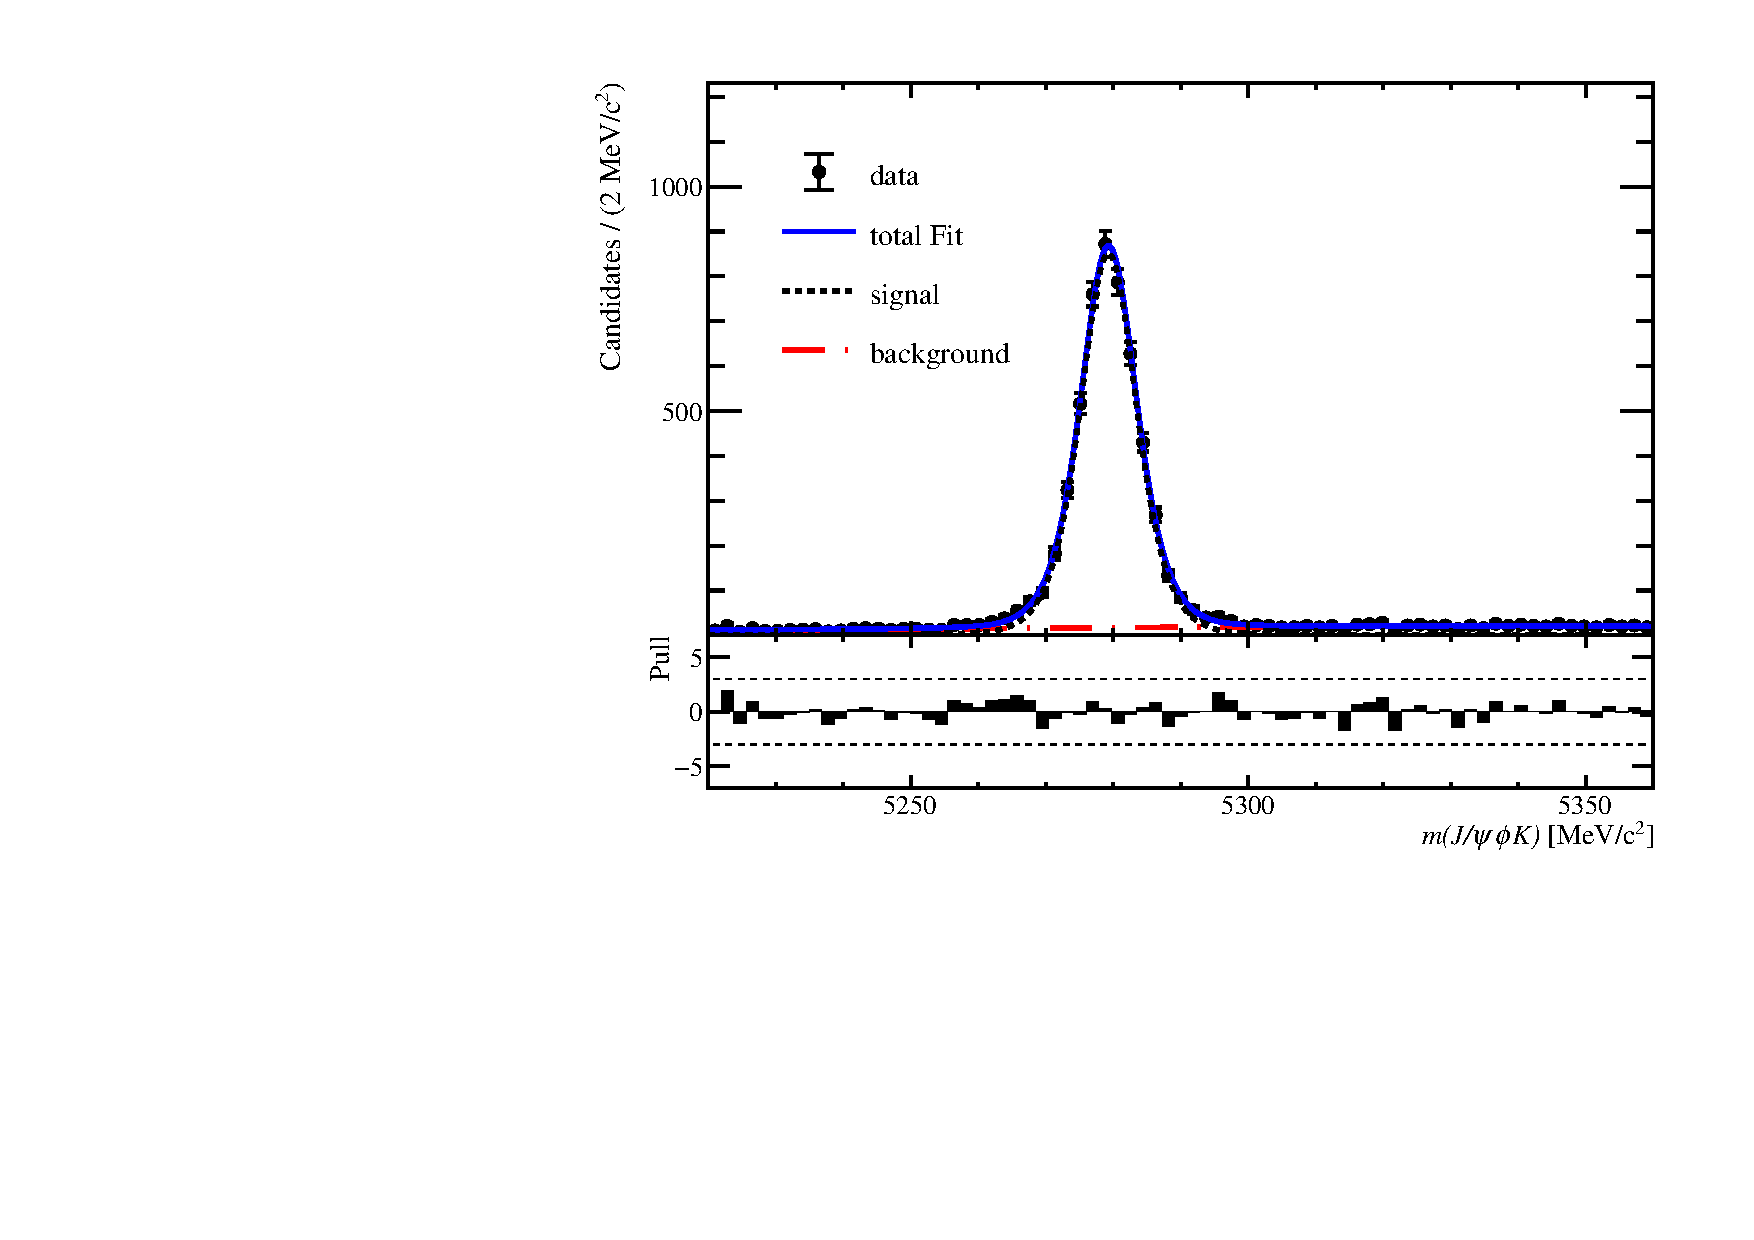
\includegraphics[width=0.75\textwidth]{Figures/03_Zcs/04_Selection/fitall_mass_JpsiKKK_sbkg_run1}
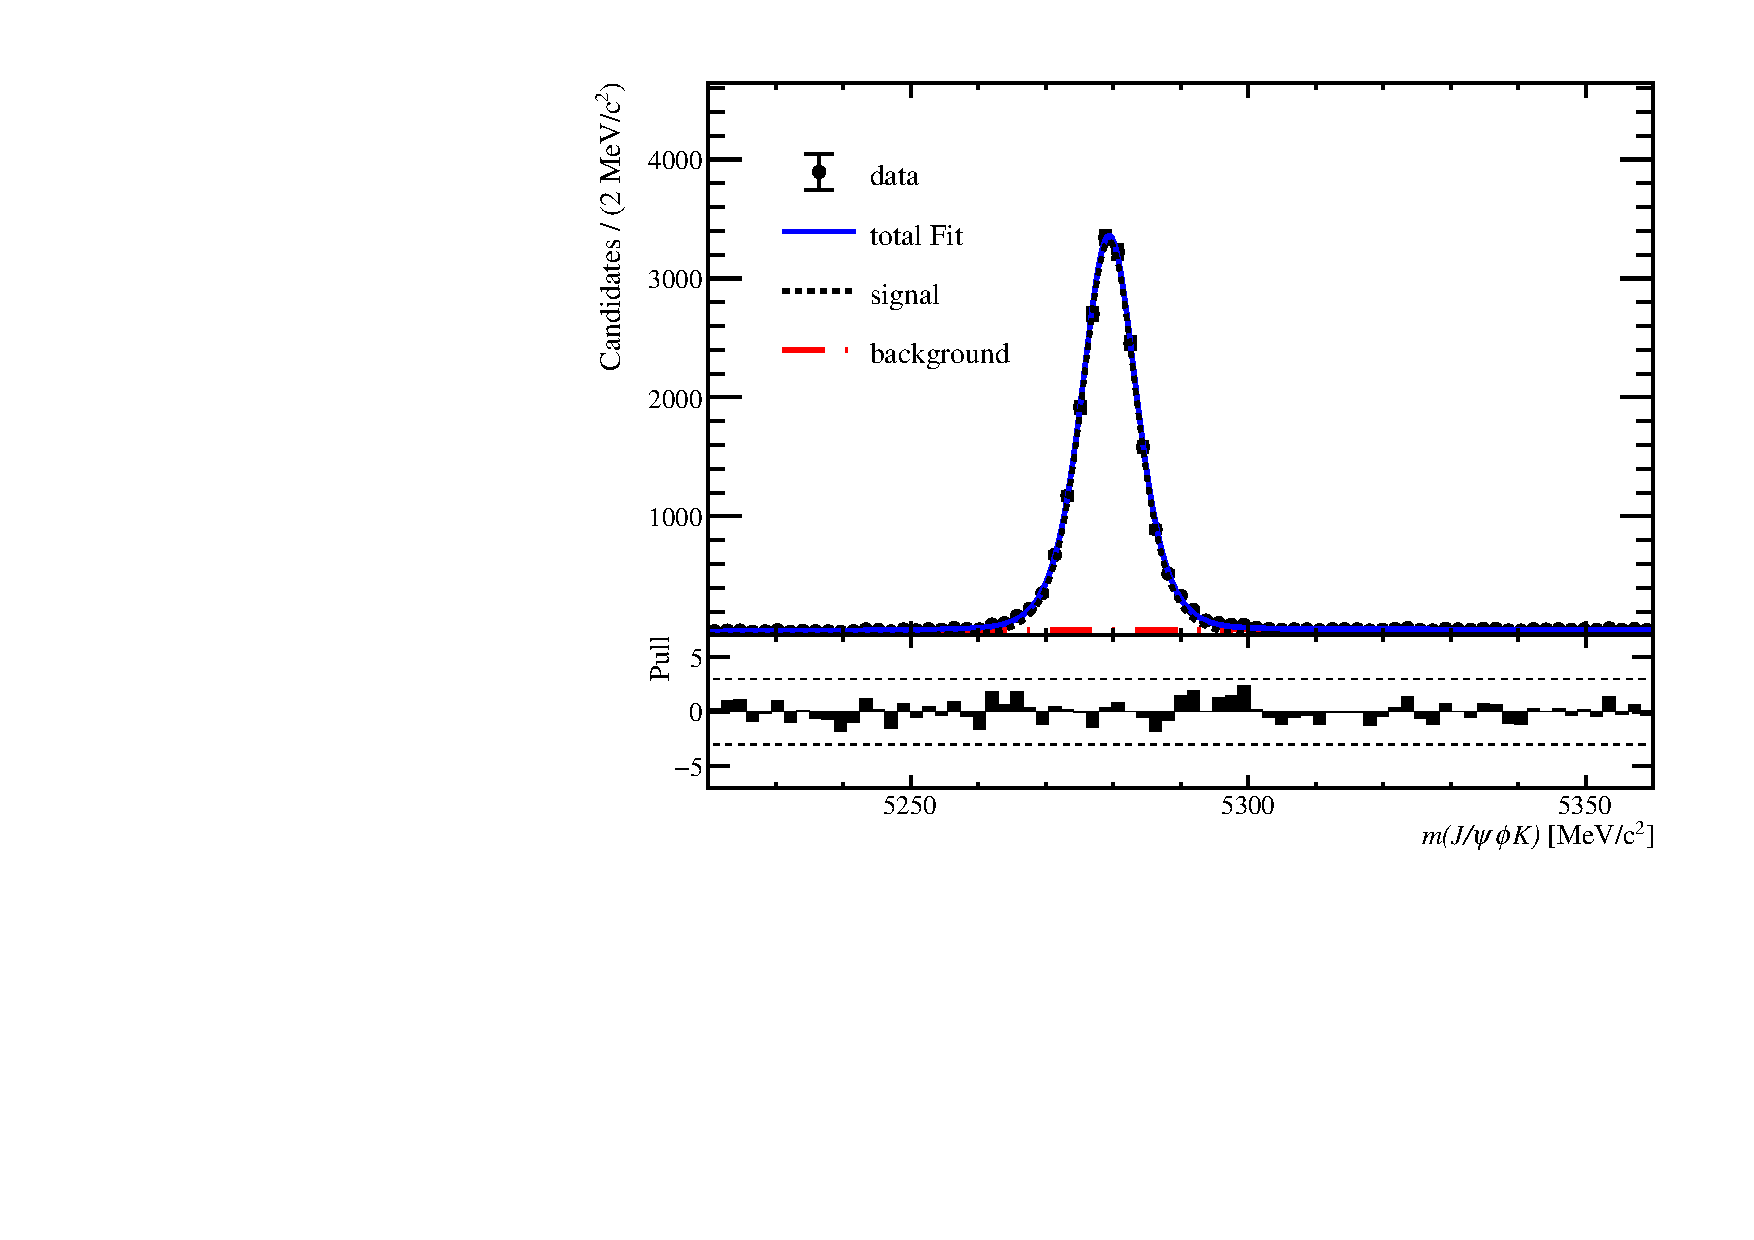
\includegraphics[width=0.75\textwidth]{Figures/03_Zcs/04_Selection/fitall_mass_JpsiKKK_sbkg_run2}
\caption{Invariant mass distribution of the $\Bpdecay$ decay and the fitted curve for Run 1 (top) and Run 2 (bottom).} 
\label{fig:MassFit_run}
\end{figure}
%%%%%%%%%%%%%%%%%%%%%%%%%%%%%%%%%%%%%%%%%%%%%%%%%%%%%%%%%%%%%%%%%%%%%%%%%%%%%%%%%%%%%%%%%%%%%%%%%%%%%%%%%%%%%%%%%%%%%%%

%%%%%%%%%%%%%%%%%%%%%%%%%%%%%%%%%%%%%%%%%%%%%%%%%%%%%%%%%%%%%%%%%%%%%%%%%%%%%%%%%%%%%%%%%%%%%%%%%%%%%%%%%%%%%%%%%%%%%%%
\begin{figure}[!tbp]
\centering
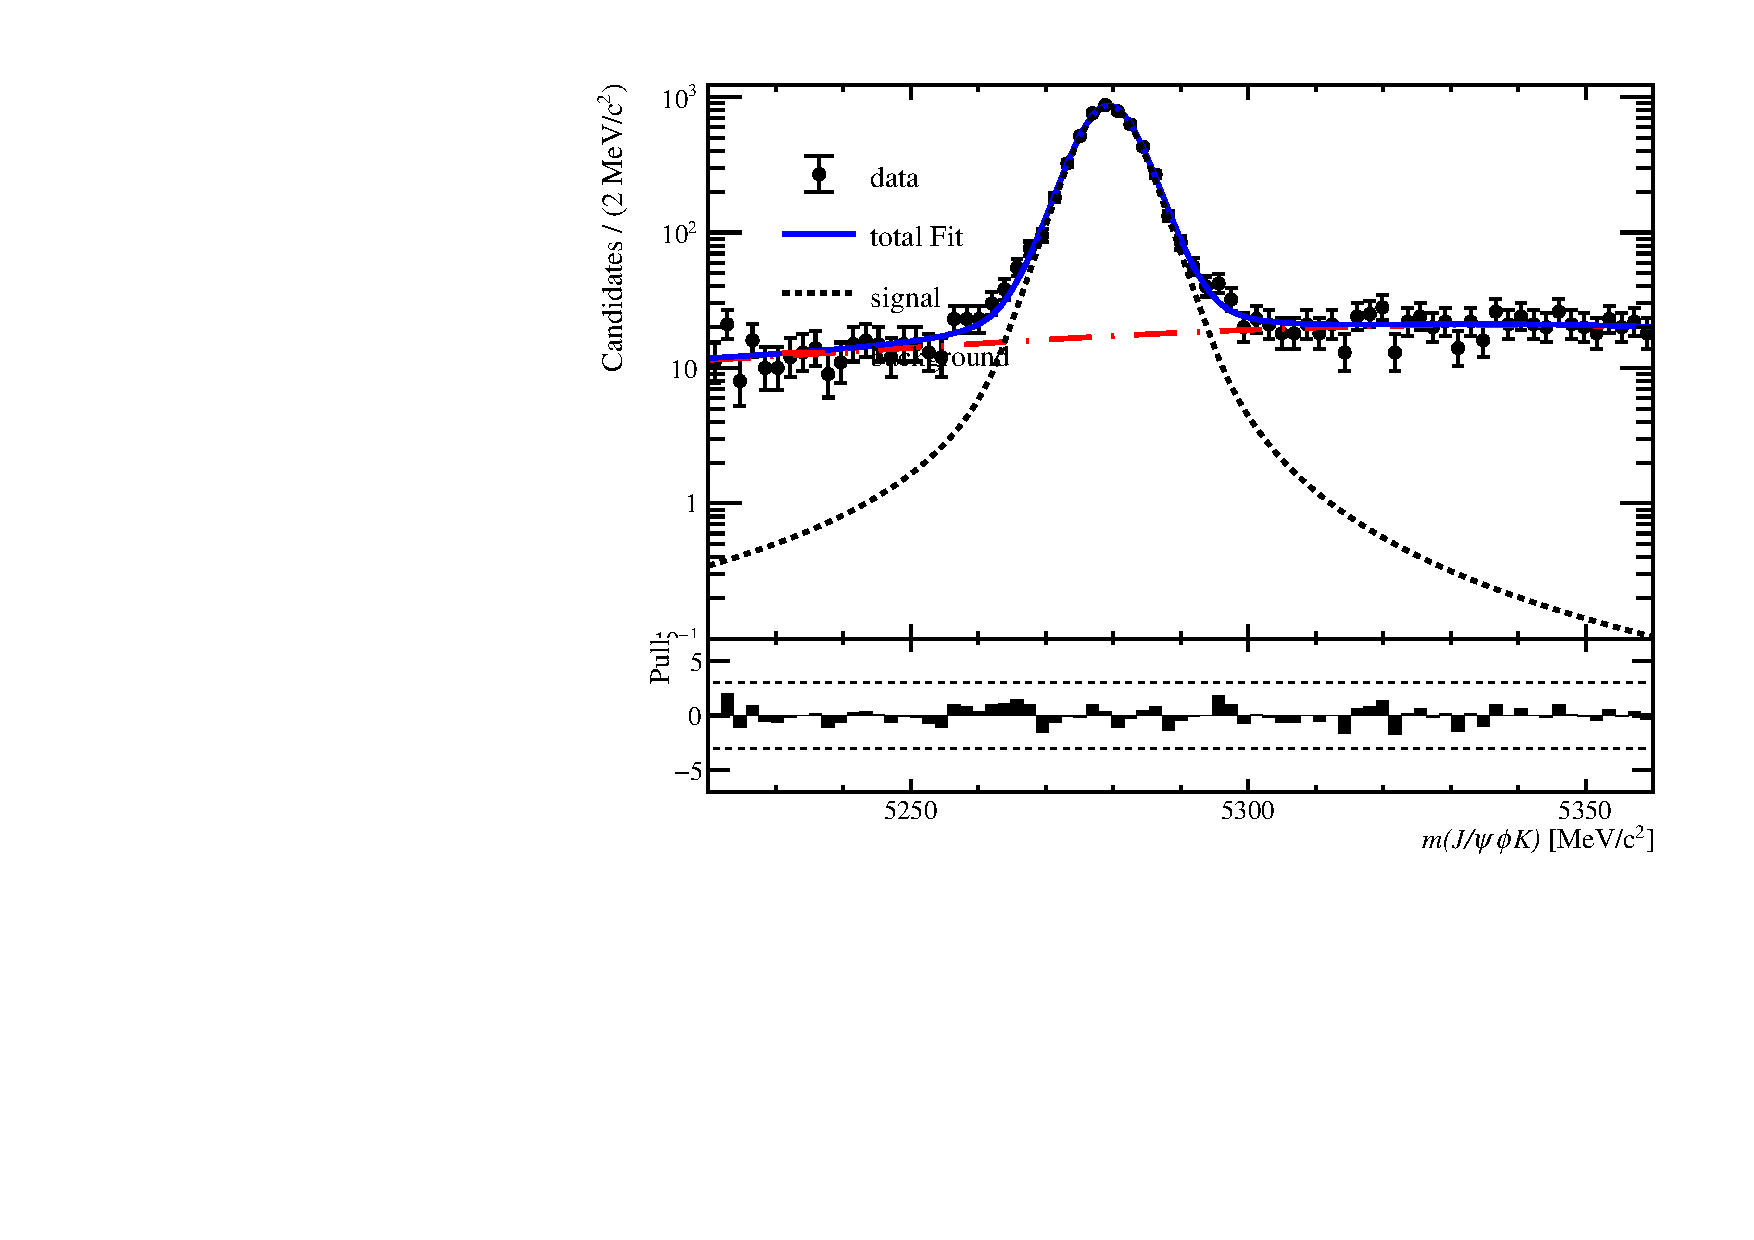
\includegraphics[width=0.75\textwidth]{Figures/03_Zcs/04_Selection/fitall_mass_JpsiKKK_sbkg_run1_log}
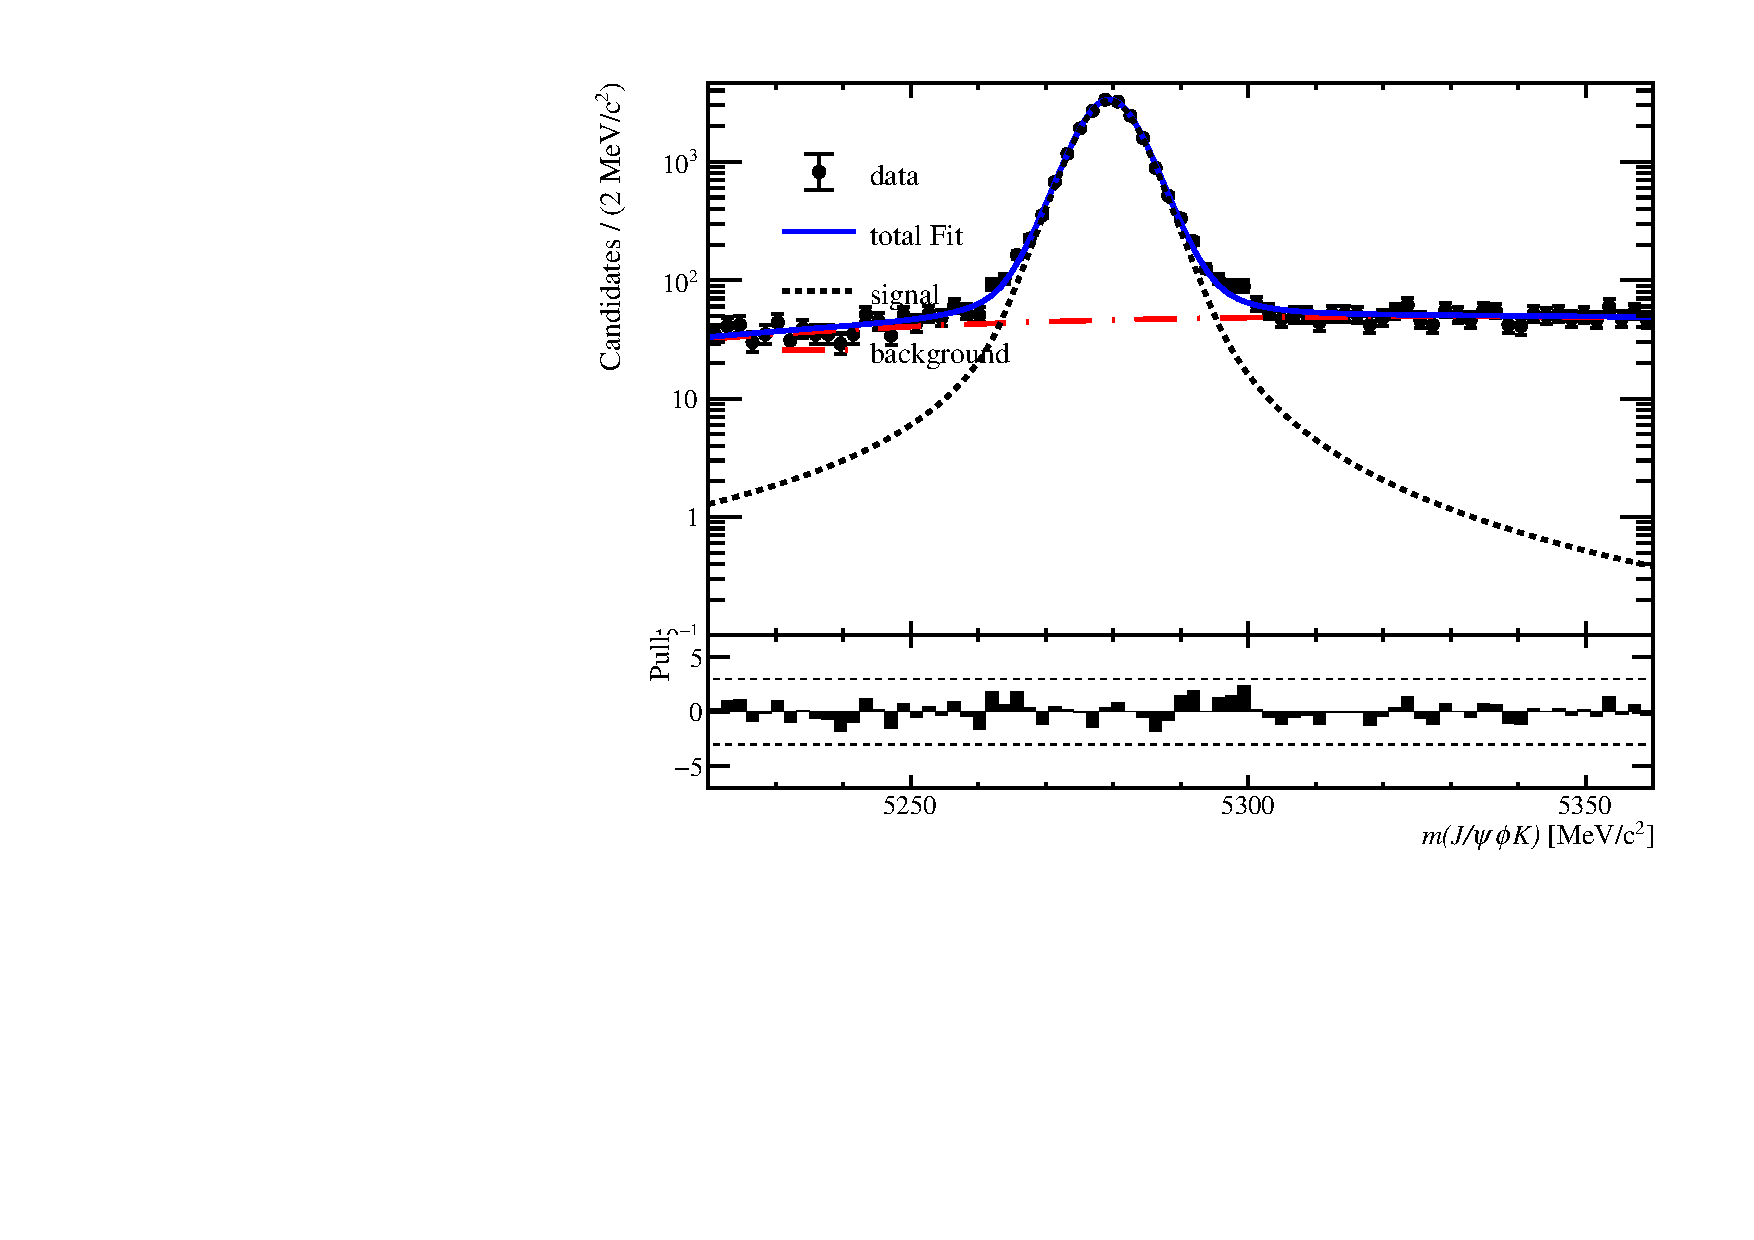
\includegraphics[width=0.75\textwidth]{Figures/03_Zcs/04_Selection/fitall_mass_JpsiKKK_sbkg_run2_log}
\caption{The log scale invariant mass distribution of the $\Bpdecay$ decay and the fitted curve for Run 1 (top) and Run 2 (bottom).} 
\label{fig:MassFit_run_log}
\end{figure}
%%%%%%%%%%%%%%%%%%%%%%%%%%%%%%%%%%%%%%%%%%%%%%%%%%%%%%%%%%%%%%%%%%%%%%%%%%%%%%%%%%%%%%%%%%%%%%%%%%%%%%%%%%%%%%%%%%%%%%%

Figure.~\ref{fig:dp1}-\ref{fig:dp3} show three Dalitz plot distributions, 
with the background subtracted by \sPlot technique.
The sWeightes are determined by the fits displayed in Figure.~\ref{fig:MassFit_run}.
The log scale mass distribution is shown in Figure.~\ref{fig:MassFit_run_log}.
The most apparent features are four bands in $\jpsi \phi$ mass, 
corresponding to $\Xone$, $\Xtwo$, $\Xthree$ and $\Xfour$ claimed in the previous LHCb publication. 
No apparent structures in $\phi K$ mass are seen, 
as many $K^*$ resonances in this mass range are broad and overlapping.
The increased data sample reveals clustering of events in the middle part of the Dalitz plots, 
best described as $\jpsi K$ mass band.
 
\begin{figure}[!tbp]
\centering
\begin{minipage}[t]{0.73\textwidth}
\centering
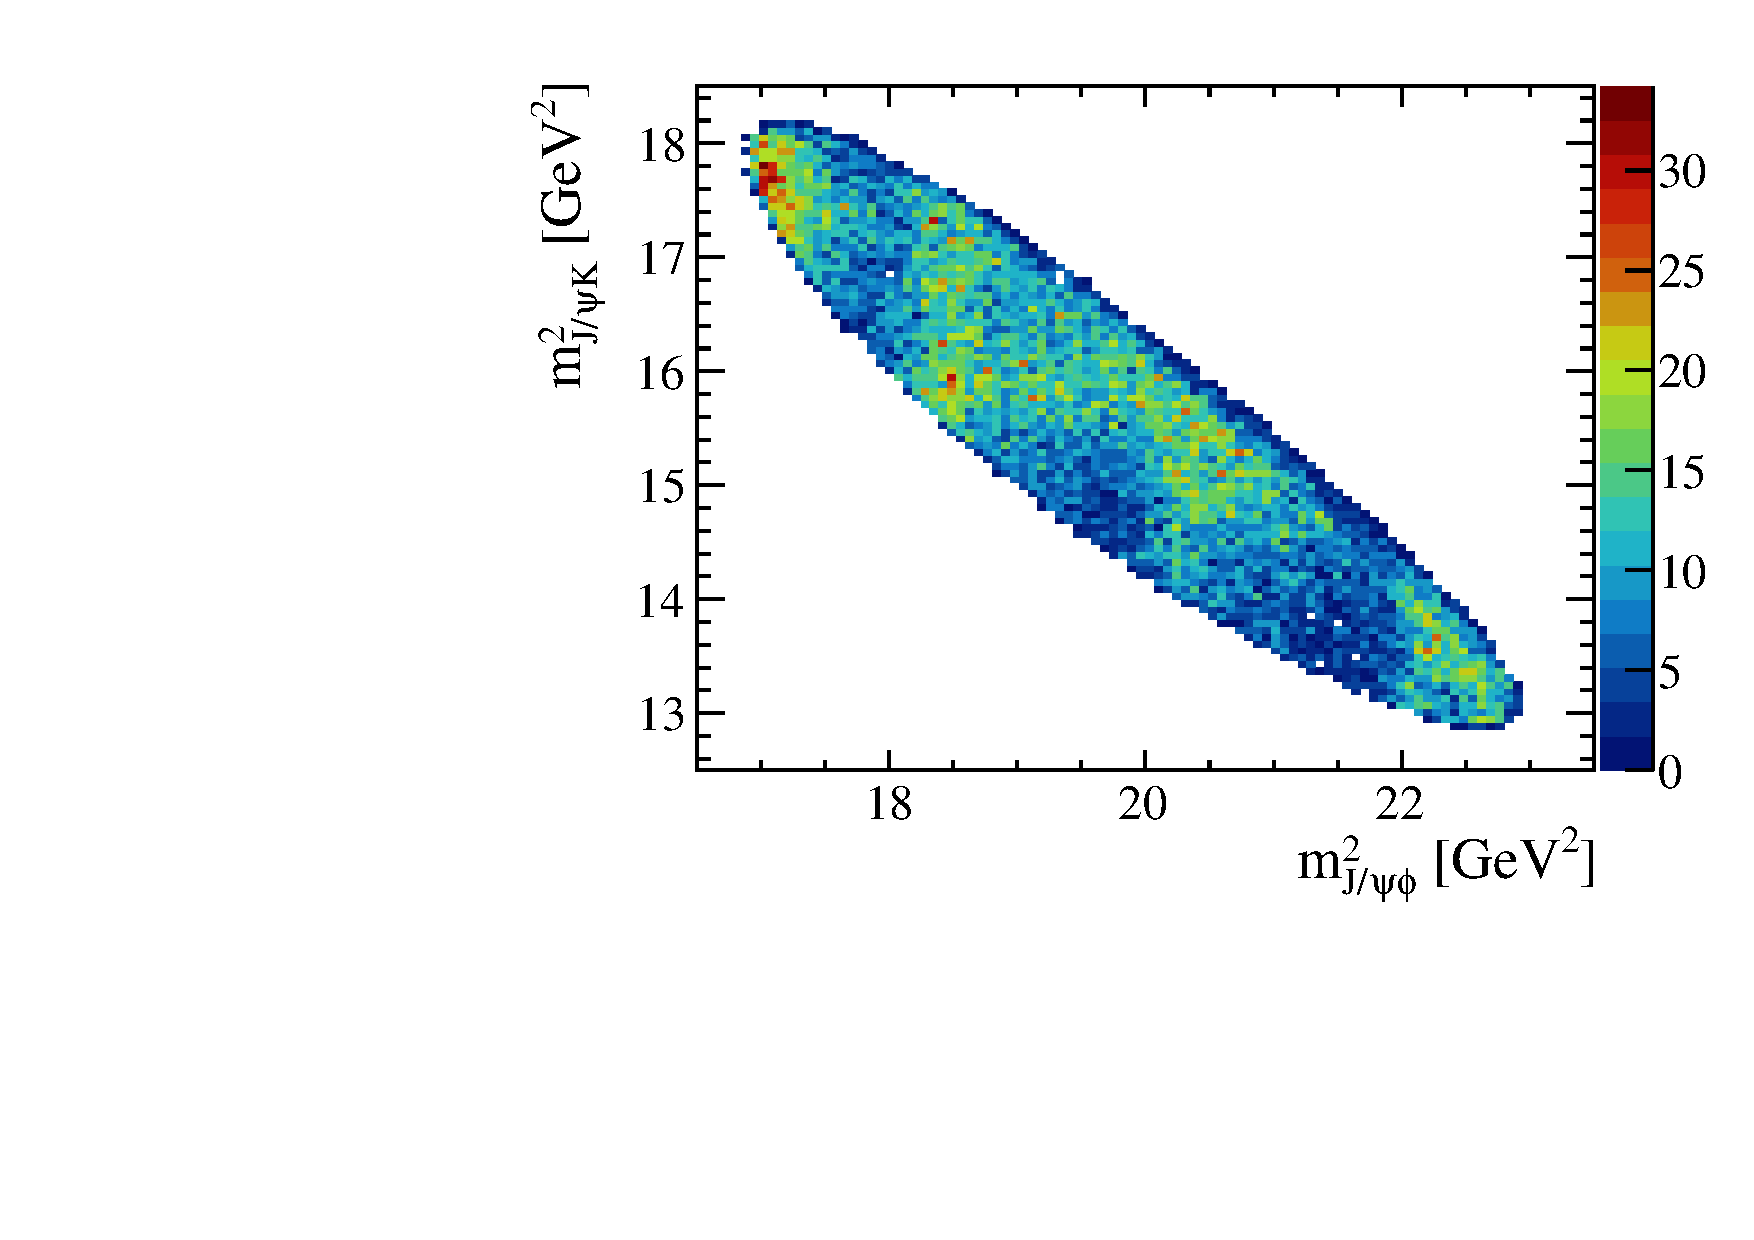
\includegraphics[width=1.0\textwidth]{Figures/03_Zcs/04_Selection/mjpsik2_mjpsiphi2}
\end{minipage}
\caption{Dalitz-plot distribution of $\jpsi\phi$ vs $\jpsi K$, where the background is subtracted by \sPlot technique.} 
\label{fig:dp1}
\end{figure}

\begin{figure}[!tbp]
\centering
\begin{minipage}[t]{0.73\textwidth}
\centering
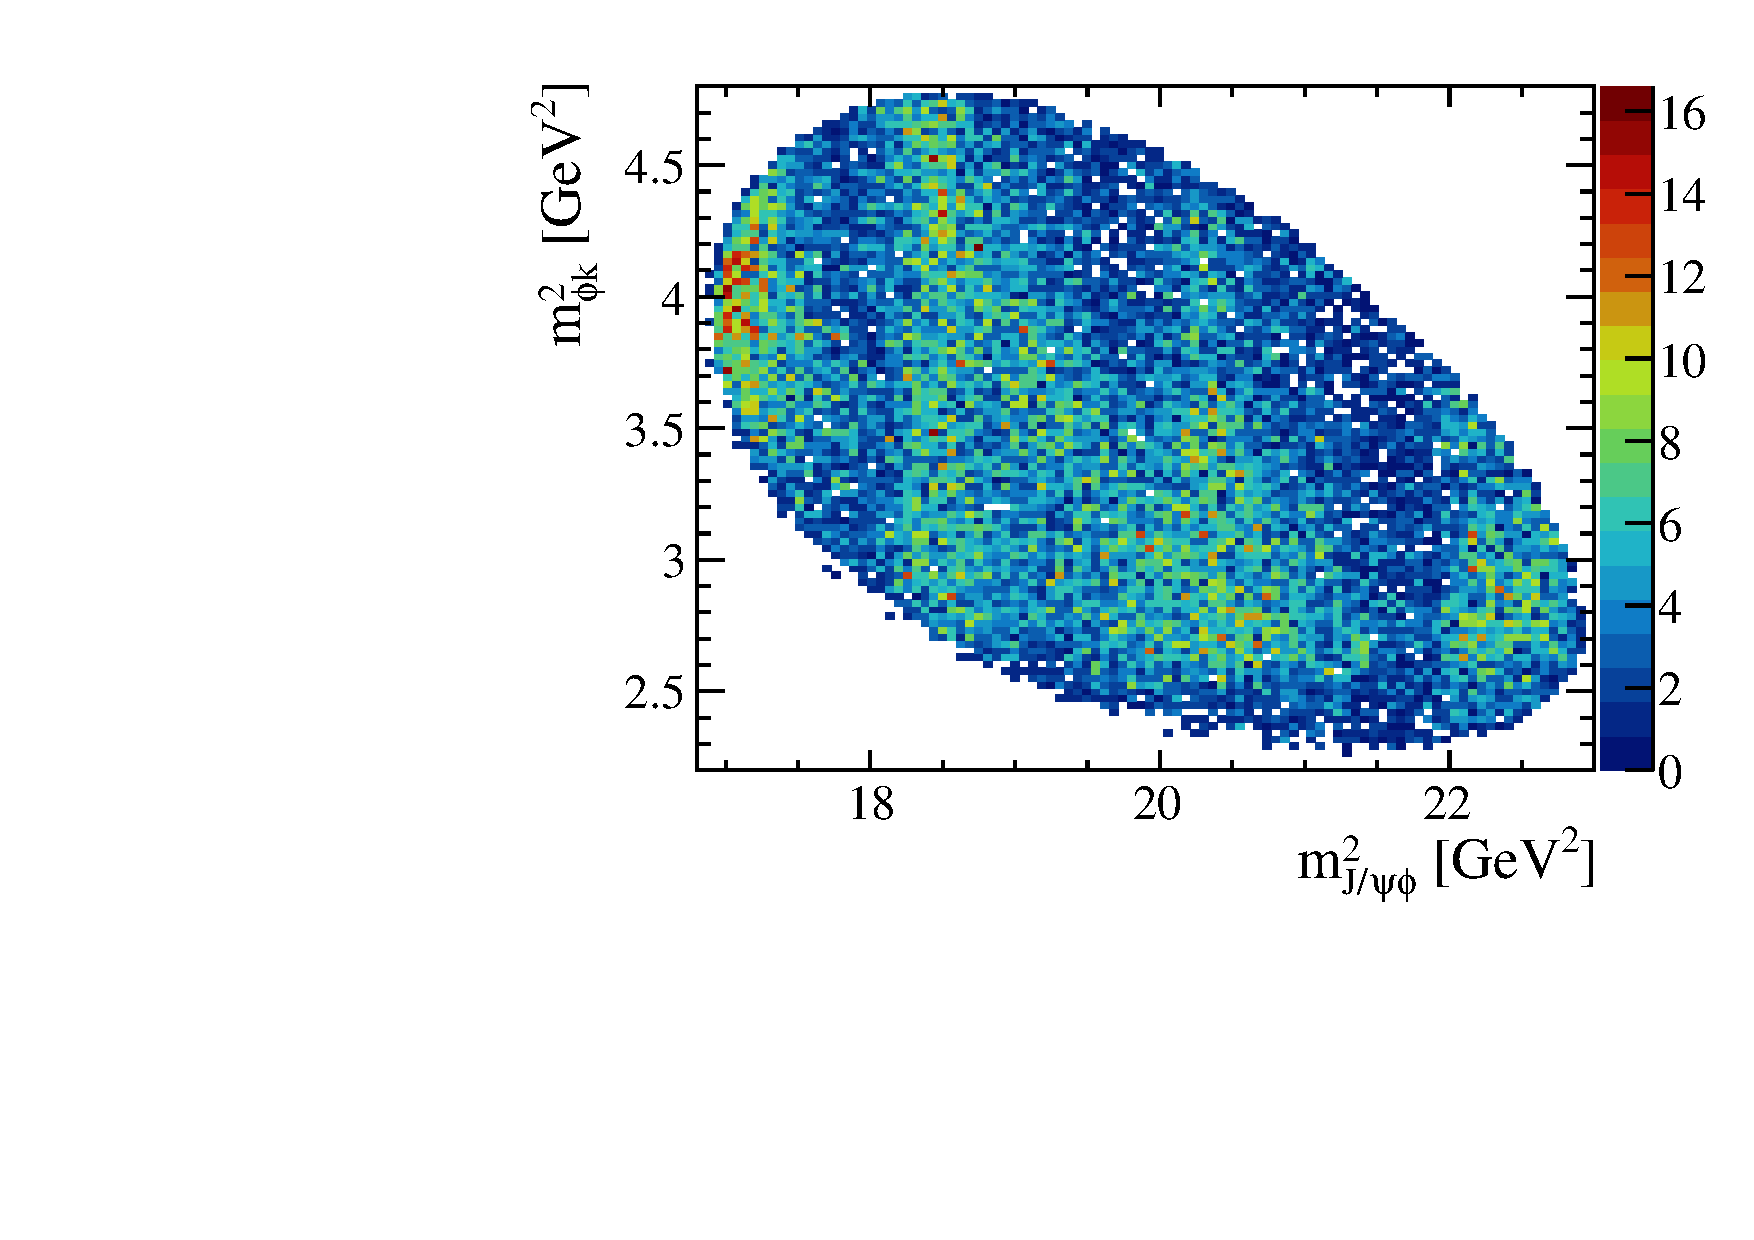
\includegraphics[width=1.0\textwidth]{Figures/03_Zcs/04_Selection/mphik2_mjpsiphi2}
\end{minipage}
\caption{Dalitz-plot distribution of $\jpsi\phi$ vs $\phi K$, where the background is subtracted by \sPlot technique.} 
\label{fig:dp2}
\end{figure}


\begin{figure}[!tbp]
\centering
\begin{minipage}[t]{0.73\textwidth}
\centering
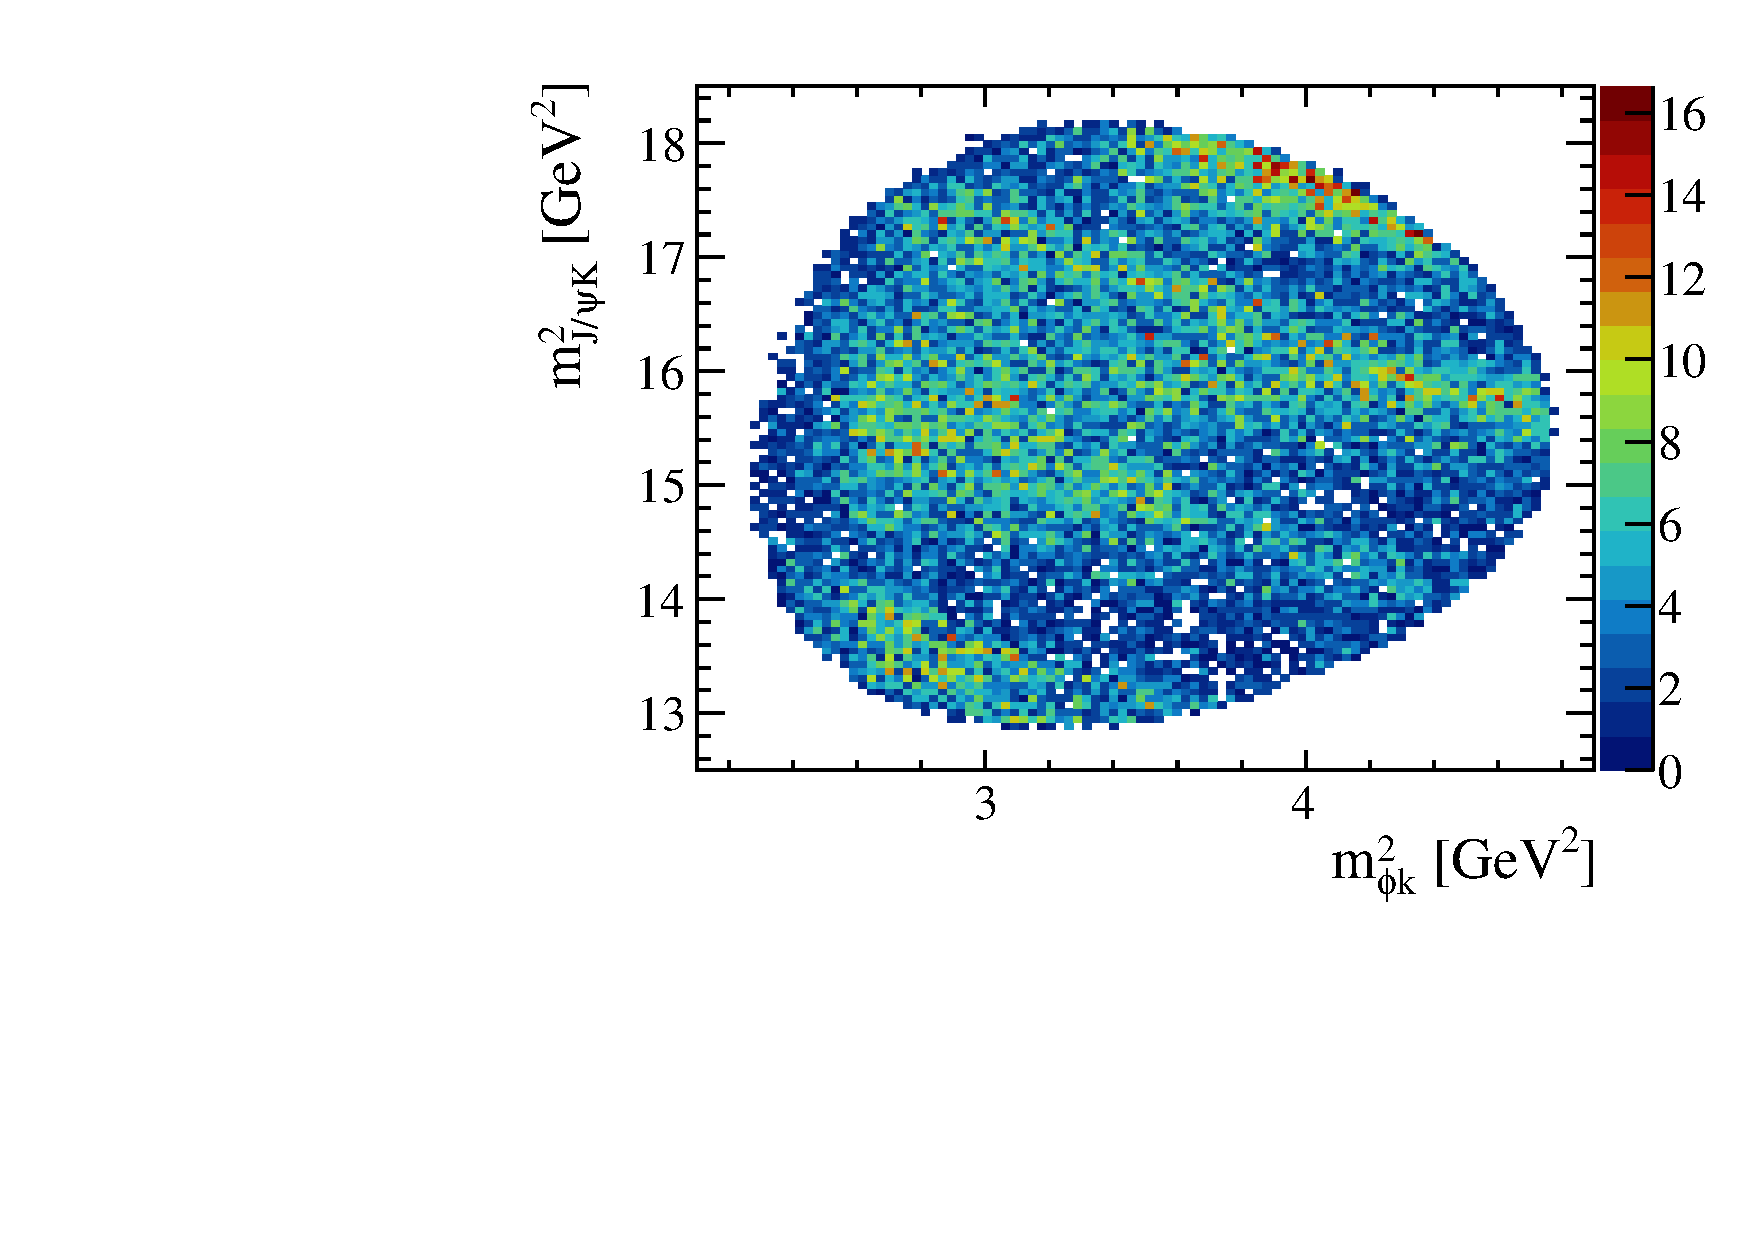
\includegraphics[width=1.0\textwidth]{Figures/03_Zcs/04_Selection/mjpsik2_mphik2}
\end{minipage}
\caption{Dalitz-plot distribution of $\phi K$ vs $\jpsi K$ , where the background is subtracted by \sPlot technique.} 
\label{fig:dp3}
\end{figure}


\subsection{Non-$\phi$ background fraction}
\label{SUPPsec:app_mphi_mB_2D_fit}
In this subsection, 
the non-$\phi$ background fraction in the total $\Bp\to\jpsi\Kp\Km\Kp$ decays with $m_{\Kp\Km}$ in $\pm$15\mev around the $\phi$ peak is estimated.
To recover proper $\phi$ mass sideband, 
the one-phi selection requirement is removed.
Later the efficiency of the one-phi cut using signal simulation is studied.
A 2D fit to $m_{\Kp\Km}$ versus $m_{\jpsi \Kp\Km\Kp}$ (2 entries per event) is done to Run 1 $+$ Run 2 data sample.
The fit result is shown in Figure.\ref{fig:app_2D_fit}.

\begin{figure}[!hbtp]
\centering
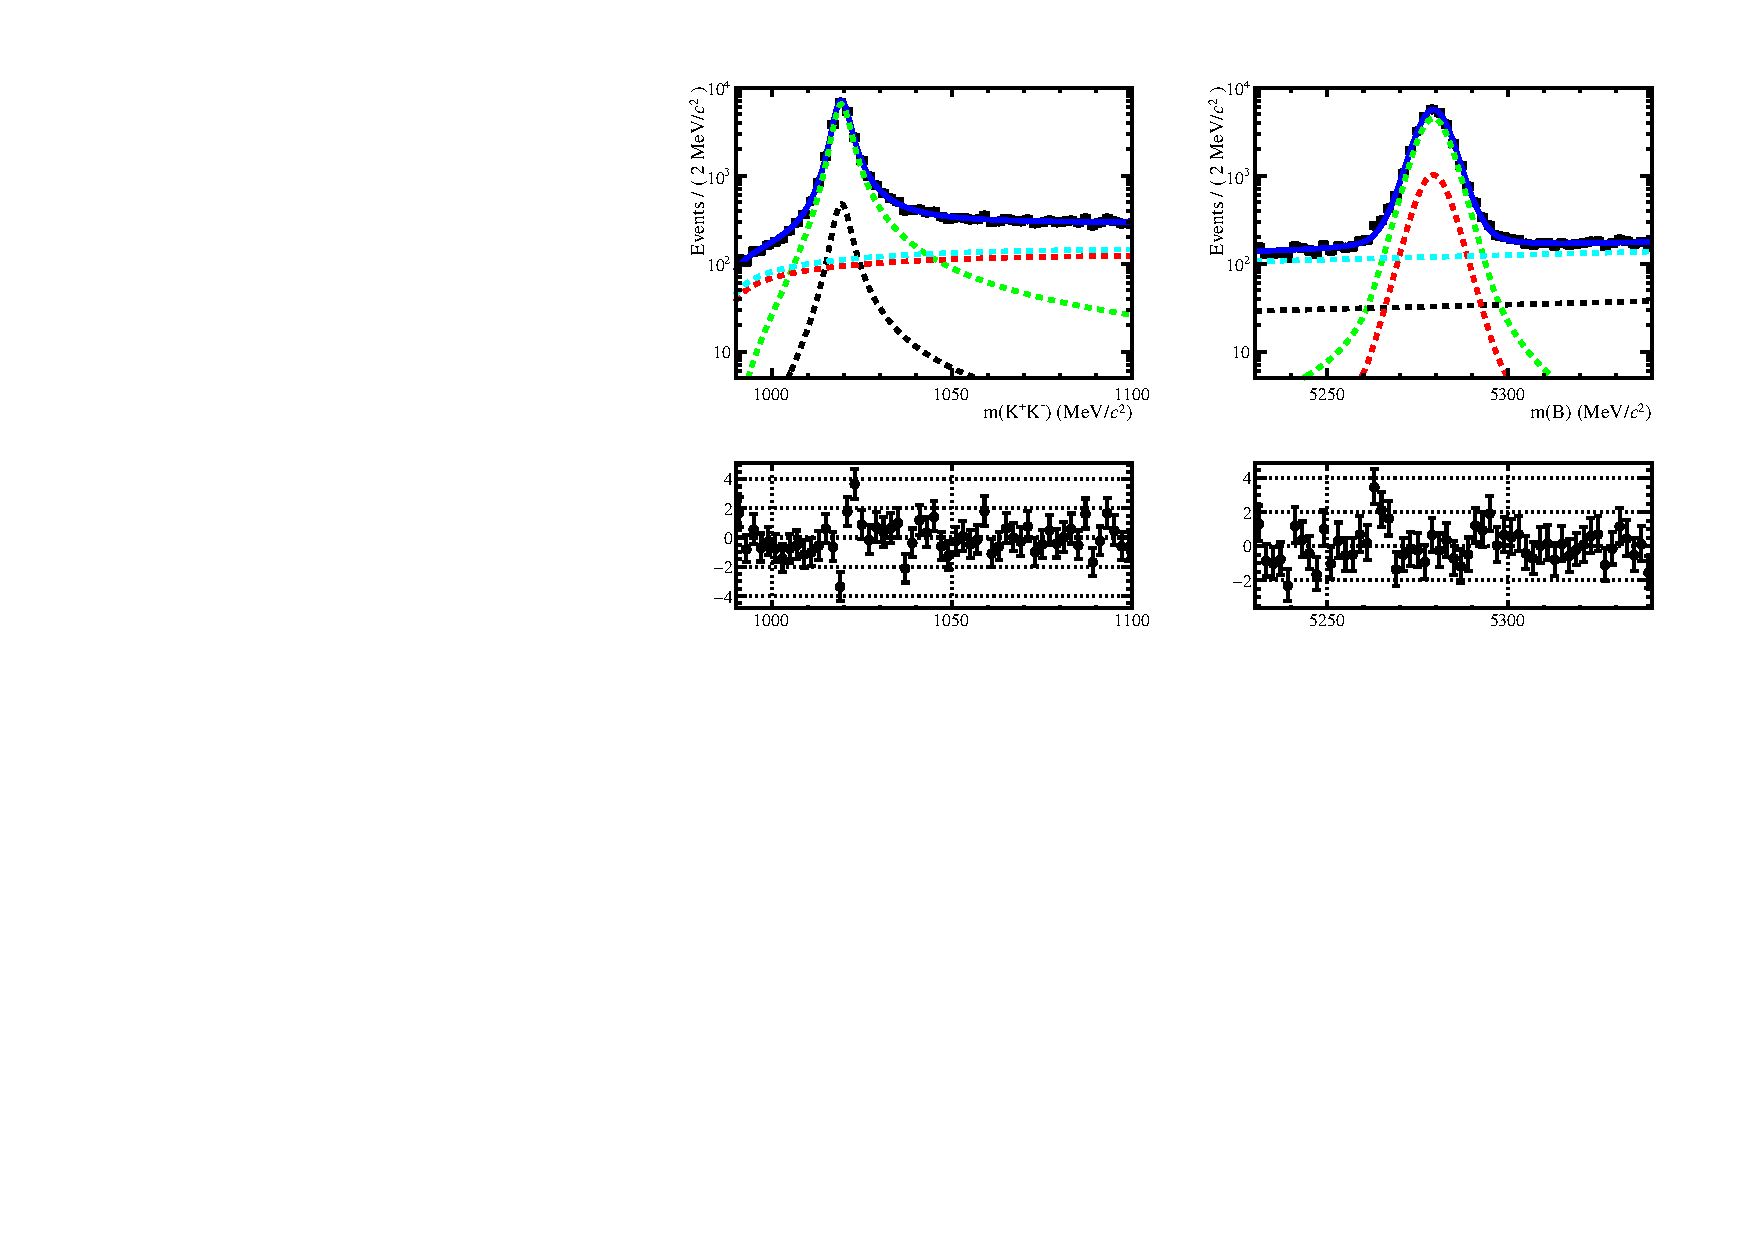
\includegraphics[width=1.\textwidth]{Figures/03_Zcs/04_Selection/app_2Dfit_mphi_mB.pdf}%
\caption{Projections of the 2D fit to $m_{\phi}$ vs.\ $m_{\jpsi\Kp\Km\Kp}$ (notice the log scale!).
  The deep blue line is the total pdf.
  The red line is the component where phi is background (modelled by phase-space) but \Bpm is signal (hypathia function).
  The green line is the component where phi is signal (Breit-Wigner) and \Bpm is signal as well.
  The black line is the component where phi is signal but \Bpm is background (linear polynomial). 
  The light blue line is the component where phi and \Bpm are both background.}
\label{fig:app_2D_fit}
\end{figure}

The yields of different fit components are shown in Table.\ref{table:app_yilds_of_2D_fit}.
Without the one-phi cut, 
the non-$\phi$ contribution in $\Bp\to\jpsi\Kp\Km\Kp$ decays is  $1366/(22018+1366)=5.8\%$ in the $\pm15\mev$ region around the $\phi$ and the $\Bp$ mass peaks.
According to the signal simulation, 
the real $\phi$ decays can generate combinatorial background in $\pm$15\mev around the $\phi$ mass peak, 
via the second $K^+K^-$ combination in the event, in a rate of 3.6 per 100 detected $\phi$ signal counts. 
This means $3.6/100 * 22018 =  793$ entries in the $\phi$ peak region are the reflections from $\phi$ signal. 
With the one-phi requirement, 
94\% of such non-$\phi$ combinations are rejected, 
with a $\phi$ signal efficiency of 97\%.  
The remaining $\phi$ signal is $22018*97\%=21357$, 
and the remaining non-phi background is $(1366-793)+(793*6\%)=621$, 
thus $621/(621+21357)=2.8\%$ is the non-$\phi$ component in the $\Bp\to\jpsi\Kp\Km\Kp$ signal sample after the one-phi requirement. 
We have assumed above that the non-phi background efficiency is 100\% for the one-phi requirement. 
Otherwise, the estimate is even lower than 2.8\%.
\begin{table}[h]
\begin{center}
\caption{The yields of 2D fit.}
\label{table:app_yilds_of_2D_fit}
\begin{tabular}{ccc}
\hline
Yields &  in fit region  &in $\pm15\mev$ of both $\phi$ and $\Bp$ signal region \\
\hline
$\phi_{signal} \otimes B_{signal}$         & $ 24826\pm185 $   &$22018\pm 164$\\
$\phi_{signal} \otimes B_{background}$     & $ 1823 \pm 81 $   &$442 \pm 20$\\
$\phi_{background} \otimes B_{signal}$     & $ 5644 \pm 124$   &$1366 \pm 30$\\
$\phi_{background} \otimes B_{background}$ & $ 6670 \pm 109$   &$441 \pm 7$\\
\hline
\end{tabular}
\end{center}
\end{table}



